\section{Ablation Studies}
\label{app:ablations}

To isolate the impact of primary data components in \MixtureVitae{}, we define \textbf{Web} and \textbf{Instructions} subsets (see Figure~\ref{fig:composition_combined}; \textbf{Instructions} encompasses Reasoning \& Instruction and Math parts of the full mixture) and conduct an ablation study on a 100B-token scale. We train three separate models: (1) \textbf{\MixtureVitae{} (full)}, the complete dataset; (2) \textbf{\MixtureVitae{} (w/o Web)}, removing the \textbf{Web} component; (3) \textbf{\MixtureVitae{} (w/o Instructions)}, removing the \textbf{Instructions} component.

% (containing Reasoning \& Instructions and Math parts) 

The average downstream performance of these models (Figure~\ref{fig:ablate}) shows varying contributions by each component: The \textbf{Instructions} data is the most critical driver of performance, as its removal results in the largest, consistent drop of average performance compared to other configurations. Removing \textbf{Instructions} particularly leads to severe drop on GSM8k (from $0.47$ to $0.03$) and MBPP, as shown in Figure~\ref{fig:ablate_table}.  Absent the \textbf{Instructions} data, the model fails to match the gains of the full mix, underscoring the essential role of instruction-following data in generalization.

Removing the \textbf{Web} component (\textbf{w/o Web}, blue dashed line) also results in a performance drop below the full dataset, albeit less dramatically. Figure~\ \ref{fig:ablate_table} shows a drop from $0.47$ to $0.41$ on GSM8k, far less severe than the drop close to $0$ for \textbf{w/o Instructions} and only slight changes on code evals. The comparison of ablation effects again highlights the \textbf{crucial role of instruction and reasoning data in achieving high performance}.

% The \texttt{Web} component shows better value than \texttt{Curated}.

% (which includes Reasoning \& Instruction and Math parts of full mixture)
% tab:eval_ablations_math_code
% Additional experiments on 80BT show that

% Counter-intuitively, the \texttt{w/o Curated} model (orange, dashed line) achieved the \textbf{highest performance}, outperforming the full \MixtureVitae{} dataset. Also on GSM8k, HumanEval and MBPP, removing \texttt{Curated} improves performance. This suggests that at 100B token scale, the \texttt{Curated} component introduces data that deteriorates the dataset composition quality.


%  when compared to the signal from the \texttt{Web} and \texttt{Instructions} components
%This finding suggests that simply adding more high-quality curated data does not guarantee improved performance, and that the interaction between diverse data sources is a key factor in optimization.




\begin{figure}[htbp]
    \centering
     \begin{subfigure}[c]{0.48\textwidth}
        \centering        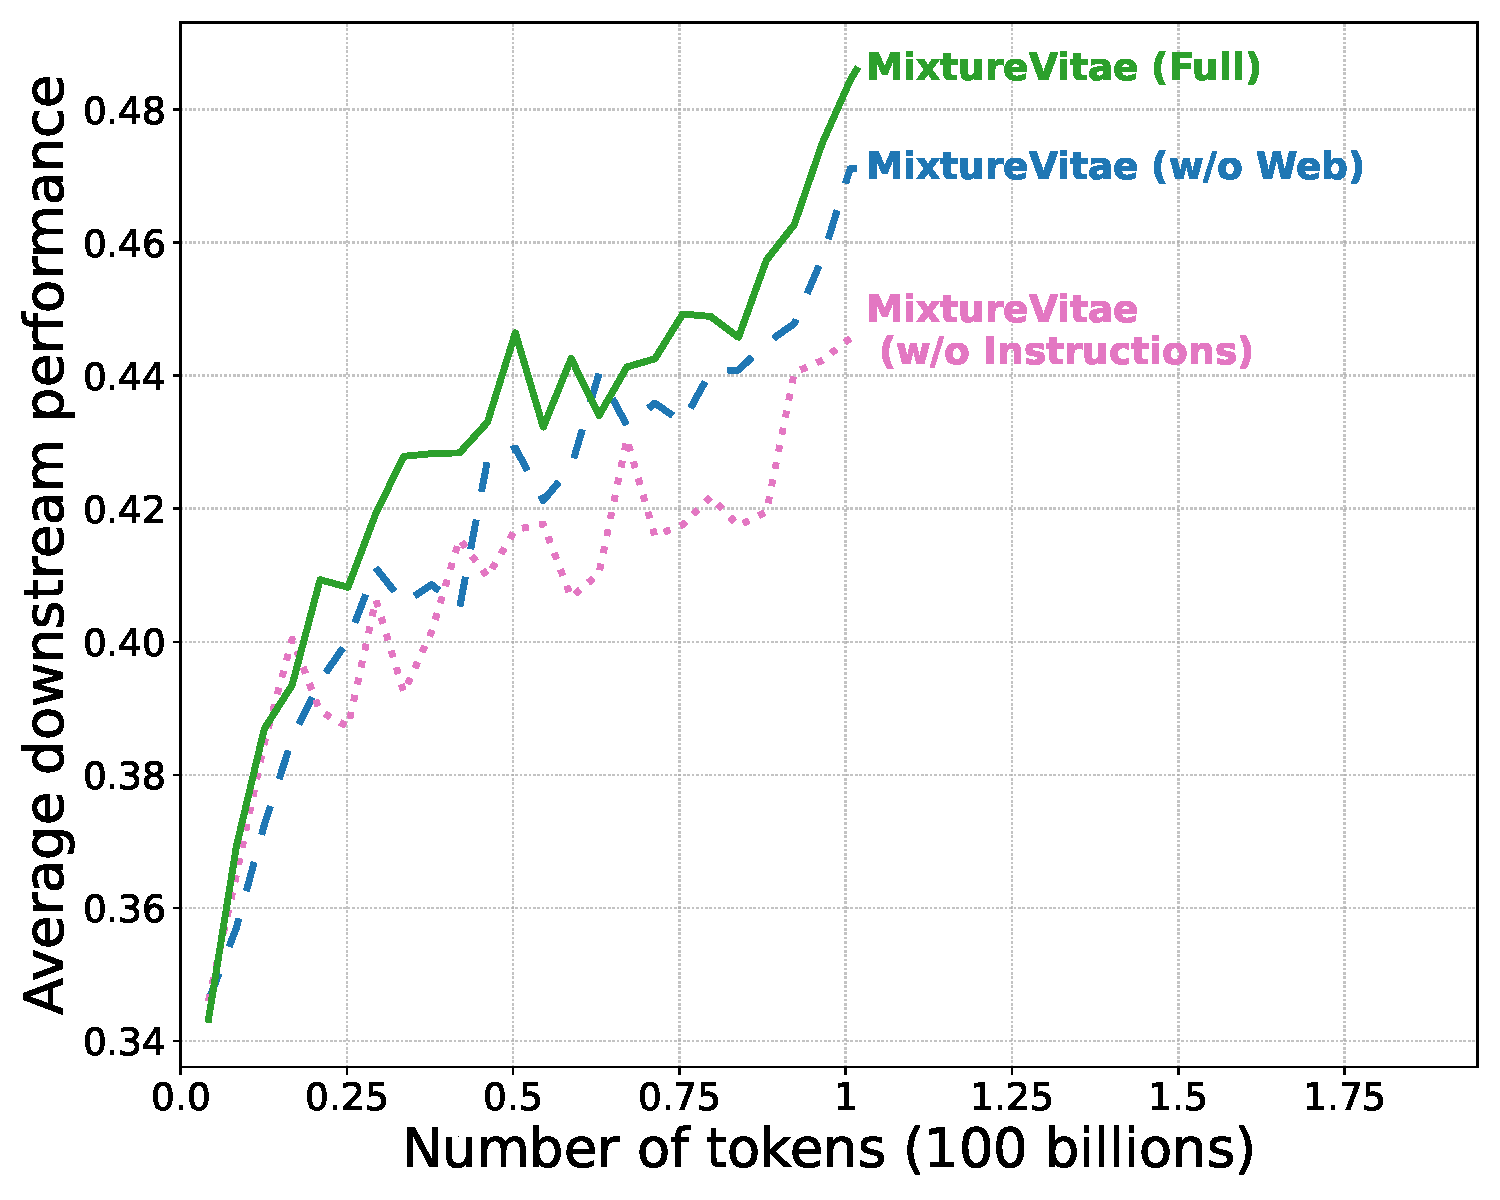
\includegraphics[width=\linewidth]{figures/Average_Performance_vs_Tokens_curated_instruct,web_instruct,web_curated,full_.pdf}
          \caption{Ablation on full \MixtureVitae{} against two versions, each excluding a data subset as indicated by \texttt{w/o}. Average performance on 10 downstream tasks.}
        \label{fig:ablate}
    \end{subfigure}%
\begin{subfigure}[c]{0.48\textwidth}
\centering

\caption{A performance breakdown on math, coding and instruction following tasks for the ablated dataset variants. Best results are in \textbf{bold}. Numbers in \textcolor{red}{red} indicate strong performance drop.}

% Updated column specification from llrrrrrrrr to llrrrr
\resizebox{1\linewidth}{!}{
\begin{tabular}{lrrrr}
\toprule
Training Dataset  & IF-Eval & GSM8K & MBPP & Average \\
\midrule
\MixtureVitae{} & 0.14 & \textbf{0.47} & \textbf{0.34} & \textbf{0.25} \\
\shortstack{\MixtureVitae{}\\(w/o Web)} & 0.18 & 0.41 & 0.33 & \textbf{0.25} \\
\shortstack{\MixtureVitae{} \\ (w/o Instructions)} & \textbf{0.19} & \textcolor{red}{0.03} & \textcolor{red}{0.14} & 0.14 \\
\bottomrule
\end{tabular}}
\label{fig:ablate_table}
\end{subfigure}
 \caption{An ablation study on components of the \MixtureVitae{} dataset. Figure~\ref{fig:ablate} shows performance average on 10 downstream evals during training, while Figure~\ref{fig:ablate_table} shows scores on further separate math, code and instruction benchmarks. The evaluation setup is given in Table~\ref{tab:reasoning-eval-settings}.}
\label{fig:ablate_all}
\end{figure}

% Figure~\ref{fig:avg_performance} shows the average performance across all 10 benchmarks of the reference models trained on different datasets at the 300B token scales. Non-permissive datasets, particularly Nemotron-CC-HQ and DCLM, still achieve the highest overall performance. %However, towards the later stages of training, MixtureVitae closely approaches these less permissive, high-risk baselines and even surpasses FineWeb-Edu, a strong non-permissive dataset and achieving performance comparable to the even stronger DCLM dataset. We argue that \MixtureVitae{} is the first permissive dataset to close the gap with top-tier non-permissive references. 
% More importantly, while the top-performing models are still trained on non-permissive datasets like Nemotron-CC-HQ and DCLM, our results demonstrate that this performance gap is no longer a mandate. Mixture Vitae proves that a dataset built on a fully permissive, risk-mitigated foundation can achieve highly competitive results—significantly outperforming all other permissive baselines and landing within a small, practical margin of top-tier, legally-ambiguous corpora. This finding directly challenges the prevailing assumption that reliance on high-risk, indiscriminately scraped copyrighted data is a prerequisite for training capable LLMs.

%A per-benchmark analysis at the 1.7B model scale (Figure~\ref{fig:per_dataset_performance}) reveals that \MixtureVitae{}--with pretraining alone--is capable of reasoning and instruction following, capabilities that would usually require more effort after pretraining. This can be seen most clearly in \MixtureVitae{}'s performance on MMLU, where none other performs better. Moreover, while most other baseline datasets yield performance near random chance, \MixtureVitae{} shows a distinct and steady learning curve, distinguishing it as one of the only datasets effective for this complex benchmark. \footnote{While fluctutating early on, Nemotron-CC-HQ performs better at the very end indeed. Additionally, \MixtureVitae{} has a consistent and a uniform increase on MMLU score, while Nemotron-CC-HQ shows an abrupt jump.} \MixtureVitae{}'s strong performance on MMLU, where most baselines perform near random chance, suggests that the inclusion of curated academic and encyclopedic sources in \MixtureVitae{} was particularly effective for instilling knowledge and reasoning into models trained on it. In contrast, \MixtureVitae{}'s performance on certain benchmarks like LAMBADA is modest, likely indicating a design trade-off: LAMBADA tests a model’s grasp of long-form narrative structures, a domain that was not the focus of our curation. This juxtaposition demonstrates that deliberate data curation has a direct and predictable impact on a model's capabilities. While conclusive comparison with instruction-tuned models calls for future work, our results suggest that high-quality pretraining can potentially narrow the performance gap between pretraining and post-training phases.


% \begin{figure}[h!] 
%     \centering
%     \includegraphics[width=0.9\linewidth]{figures/avg_perf.pdf}
%     \caption{Comparing average performance across 10 evaluation benchmarks (Copa[0], Openbookqa[0], Lambada[0], Winogrande[0], MMLU[5], Piqa[10], Arc-challenge[10], Arc-easy[10], Hellaswag[10], Boolq[10], [n] standing for few-shot number) for 8 different datasets trained using 300B tokens on different model scales. Dataset ranking is visible and consistent across model scales, with differences becoming more pronounced at larger model scales.}
%     \label{fig:avg_performance}
% \end{figure}


% \subsection{Red Teaming}

% The attack success rates (ASR) of the evaluated models are summarized in Table~\ref{tab:model_performance}, where safety was assessed using three benchmark datasets: \texttt{toxigen}\footnote{\url{https://huggingface.co/datasets/toxigen/toxigen-data}}, \texttt{do\_not\_answer}\footnote{\url{https://huggingface.co/datasets/LibrAI/do-not-answer}}, and \texttt{advbench}\footnote{\url{https://huggingface.co/datasets/walledai/AdvBench}}.
% The responses to red-teaming prompts were evaluated using the following safety classifiers:
% \begin{itemize}
%     \item \textbf{Llama Guard-8B}\footnote{\url{https://huggingface.co/meta-llama/Llama-Guard-3-8B}}: Used for do\_not\_answer and advbench evaluations. 
%     \item \textbf{toxigen\_roberta}\footnote{\url{https://huggingface.co/tomh/toxigen_roberta}}: A classifier aligned with the Toxigen dataset, used for its specific evaluation.

% \end{itemize}



% \begin{table}[ht]
% \centering
% \caption{Attack Success Rate (ASR) in \% for various models. Model A is \textbf{1.7b\_data-MixtureVitae-300BT-v1}, Model B is \texttt{1.7b\_data-Comma0.1-300BT}, Model C is \textbf{1.7b\_data-common\_corpus-eng-300BT}, and Model D is \textbf{open-sci-ref-v0.01-1.7b-nemotron-hq-300B-4096}.}
% \label{tab:model_performance}
% \begin{tabular}{lcccc}
% \toprule
% \textbf{Metric} & \textbf{Model A} & \textbf{Model B} & \textbf{Model C} & \textbf{Model D} \\
% \midrule
% toxigen      
%                & 8.07  & 9.04  & 12.77 & 10.21 \\
% do\_not\_answer 
%                & 28.22 & 24.71 & 21.62 & 20.98 \\
% advbench     
%                & 86.92 & 92.12 & 70.58 & 85.77 \\
% \bottomrule
% \end{tabular}
% \end{table}
% Model 1.7b\_data-Comma0.1-300BT exhibits the highest attack success rate on \texttt{advbench} (92.12\%), suggesting that it is most vulnerable to adversarial prompts. Model 1.7b\_data-MixtureVitae-300BT-v1 shows the greatest weakness on \texttt{do\_not\_answer} (28.22\%), meaning it more often fails to reject unsafe queries. Model 1.7b\_data-common\_corpus-eng-300BT is particularly prone to toxicity, with the highest ASR on \texttt{toxigen} (12.77\%). Model open-sci-ref-v0.01-1.7b-nemotron-hq-300B-4096 shows balanced results, with moderate vulnerability across all benchmarks, and does not stand out as the most exploitable in any single category.

% \subsection{Role of Instruction and Reasoning Data}
%\label{sec:role_of_instruction}
%\MixtureVitae{}’s performance is enhanced by the large proportion of reasoning and instruction data, as demonstrated in the ablation study in Section~\ref{app:ablations}. Removing this subset (“w/o Instructions” in Figure~\ref{fig:ablate_all}) causes a substantial degradation across tasks—far larger than the impact of removing the web component. This effect validates and extends the findings of Phi-4~\citep{abdin2024phi4technicalreport}, showing that a permissive-first, risk-mitigated, and reasoning-heavy mixture can substitute vast quantities of generic web text, particularly under constrained token budgets.